\ifdefined\ishandout
\documentclass[handout]{beamer}
\else
\documentclass{beamer}
\fi

\usepackage[frenchb]{babel}
\usepackage[T1]{fontenc}
\usepackage[latin1]{inputenc}
\usepackage{hyperref}
\usepackage{multirow}
\usepackage{listings}
\usepackage{fancyvrb}
\usepackage{tikz}
\usepackage{framed}
\usepackage{algorithm}
\usepackage{algorithmic}
\usepackage{xcolor}
\usepackage{color, colortbl}
\usepackage{handoutWithNotes}

\usetikzlibrary{shapes.geometric}
\usetikzlibrary{positioning}
\usetikzlibrary{shapes.arrows, chains}
\usetikzlibrary{arrows,calc}
\usetikzlibrary{shapes.multipart}
\usepackage{array}
\usetheme{Boadilla}

\ifdefined\ishandout
\pgfpagesuselayout{3 on 1 with notes}[a4paper,border shrink=5mm]
\usecolortheme{dove}
\else
\usecolortheme{dolphin}
\fi


\lstnewenvironment{codeC}
{ \lstset{language=C,
    otherkeywords={printf,scanf}}
}
{}

\ifdefined\ishandout
\definecolor{mygreen}{rgb}{0,0,0}
\definecolor{mymauve}{rgb}{0,0,0}
\definecolor{myblue}{rgb}{0,0,0}
\else
\definecolor{mygreen}{rgb}{0,0.6,0}
\definecolor{mymauve}{rgb}{0.58,0,0.82}
\definecolor{myblue}{rgb}{0,0,1}

\fi

\definecolor{mygray}{rgb}{0.5,0.5,0.5}


\lstset{language=C,
% breakatwhitespace=false,         % sets if automatic breaks should only happen at whitespace
%  breaklines=true,                 % sets automatic line breaking
%  captionpos=b,                
commentstyle=\itshape\color{mymauve},
keywordstyle=\bfseries\color{myblue},
%numbers=left,                    % where to put the line-numbers; possible values are (none, left, right)
%  numbersep=8pt,                   % how far the line-numbers are from the code
%  numberstyle=\tiny\color{mygray}, % the style that is used for the line-numbers
  rulecolor=\color{black},         % if not set, the frame-color may be changed on line-breaks within not-black text (e.g. comments (green here))
%  showspaces=false,                % show spaces everywhere adding particular underscores; it overrides 'showstringspaces'
  showstringspaces=false,          % underline spaces within strings only
%  showtabs=false,                  % show tabs within strings adding particular underscores
%  stepnumber=2,                    % the step between two line-numbers. If it's 1, each line will be numbered
  stringstyle=\color{mygreen},     % string literal style
%  tabsize=2 
}
\ifdefined\ishandout
\newcommand{\red}{\textbf}
\else
\newcommand{\red}{\textcolor{red}}
\fi
%\newcommand \emph
%Default size : 12.8 cm * 9.6 cm

\newcommand{\tmark}[1]{\tikz[remember picture, baseline=-.5ex]{\coordinate(#1);}}

\ifdefined\ishandout
\newenvironment<>{codeblock}[1]{%begin
  \setbeamercolor{block title}{fg=black,bg=lightgray!80}%
  \begin{block}{#1}}
  % \begin{codeC}}
  %  {\end{codeC}
{  
\end{block}}

\newenvironment<>{termblock}[1]{
    \setbeamercolor{block title}{fg=black,bg=lightgray!90}%
    \begin{block}{#1}
}
%     \begin{Verbatim}}
{%\end{Verbatim}
\end{block}
}

\definecolor{bluegreen}{RGB}{0,0,0}
%\definecolor{bluegreen}{rgb}{0,0.6,0.8}
\else

\newenvironment<>{codeblock}[1]{%begin
  \setbeamercolor{block title}{fg=darkgray,bg=yellow}%
  \begin{block}{#1}}
  % \begin{codeC}}
  %  {\end{codeC}
{  
\end{block}}

\newenvironment<>{termblock}[1]{
    \setbeamercolor{block title}{fg=white,bg=lightgray}%
    \begin{block}{#1}}
%     \begin{Verbatim}}
{%\end{Verbatim}
\end{block}
}

\definecolor{bluegreen}{RGB}{0,149,182}
%\definecolor{bluegreen}{rgb}{0,0.6,0.8}
\fi

%\newcommand{\output}[1]{
\setbeamertemplate{navigation symbols}{}
\newcommand{\bvrb}{\Verb[commandchars=���,formatcom=\color{bluegreen}]}
\newcommand{\footvrb}{\footnotesize\Verb}
\newcommand{\vrbalert}[2][]{\visible<#1>{#2}}
%%% Commande pour les listes/arbres
\newcommand{\mvide}{\nodepart{one} \nodepart{two}}
\newcommand{\tvide}{\nodepart{one} \nodepart{two} \nodepart{three}}

%%Fin des commandes pour les listes/arbres.



%%% Param�tres du cours (� r�gler)
%Num�ro du cours
\newcommand{\nb}{8}

\title[Cours n�\nb]{Cours n�\nb - Algorithmes avanc�s}
\author[]{julien.brajard@upmc.fr}
\institute[Polytech' UPMC]{Polytech' UPMC}
\date{16 Novembre 2015}
\begin{document}
%%%%%%%%%%%%%%%%%%%%% SLIDES DE TITRE
\begin{frame}
\titlepage
\centering{
\url{http://australe.upmc.fr} (onglet EPU-C5-IGE Info Gen)}
\end{frame}
%%%%%%%%%%%%%%%%%%%%%




%%%%%% SECTION 12
% !TEX encoding = IsoLatin9

%%%%%%%%%%%%%%%%%%%%% SECTION 1
\section{L'algorithme minimax}

\begin{frame}
\frametitle{L'algorithme minimax}
\begin{itemize}
\setlength\itemsep{1em}
\item Algorithme issu de la th�orie des jeux
\item Il s'applique aux jeux � 2 joueurs, �  somme nulle
(1 gagnant/1perdant ou match nul) et � information compl�te.
\end{itemize}

\begin{block}{Principe}
Passer en revu un nombre limit� de coups
et les �valuer en fonction du b�n�fice pour le joueur
et sont adversaire
\end{block}

\end{frame}

\begin{frame}
\frametitle{Evaluation d'un position}
\begin{columns}
\column{0.7\textwidth}
\begin{figure}
\centering
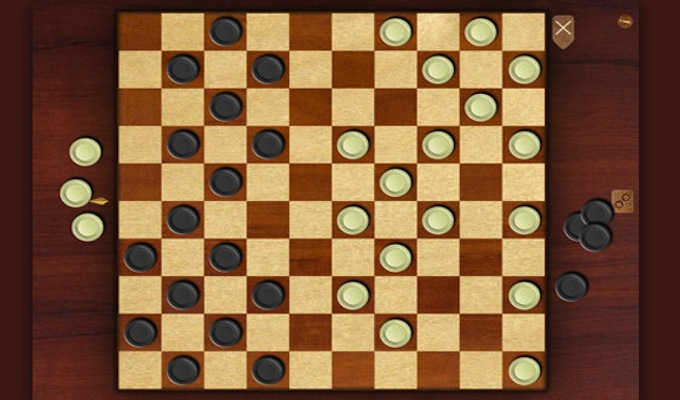
\includegraphics[width=8cm]{./fig/dames.jpg}
\end{figure}
\column{0.25\textwidth}
Joueur : Blancs\\
Adversaires : Noirs \\
\end{columns}
\vspace{1em}
Evaluation = Nbre de pions blancs - Nbre de pions noirs (ici = 1)
\end{frame}

\begin{frame}
\frametitle<1-8|handout:1-2>{Arbre minimax}
\frametitle<9-|handout:3>{Variante Negamax}
\begin{figure}
\begin{tikzpicture} [
  remember picture,
  auto,
  noeud/.style = {circle,draw=black,inner sep = 0pt, radius = 16pt,minimum size = 16pt},
  line/.style = {draw,->},
]

 \node [noeud, fill = red] (rac) {\temporal<7-8|handout:2>{}{2}{2} };

\visible<2->{ \node [noeud, fill = green, below of = rac, xshift = -2.5cm] (fg) {\temporal<6-8|handout:2>{}{0}{0} };}
\visible<2->{ \node [noeud, fill = green, below of = rac] (fm) {\temporal<6-8|handout:2>{}{2}{-2} };}
\visible<2->{ \node[noeud, fill = green, below of = rac, xshift = +2.5cm] (fd) {\temporal<6-8|handout:2>{}{-1}{1} };}

\visible<3->{ \node [noeud, fill = red, below of = fg, xshift = -0.8cm] (fgg) {\temporal<5-8|handout:2>{}{9}{9} };}
\visible<3->{ \node [noeud, fill = red,below of = fg] (fgm) {\temporal<5-8|handout:2>{}{7}{7} };}
\visible<3->{ \node [noeud, fill = red,below of = fg, xshift = 0.8cm] (fgd) {\temporal<5-8|handout:2>{}{0}{0} };}


\visible<3->{ \node [noeud, fill = red, below of = fm, xshift = -0.8cm] (fmg) {\temporal<5-8|handout:2>{}{2}{2} };}
\visible<3->{ \node [noeud, fill = red,below of = fm] (fmm) {\temporal<5-8|handout:2>{}{5}{5} };}
\visible<3->{ \node [noeud, fill = red,below of = fm, xshift = 0.8cm] (fmd) {\temporal<5-8|handout:2>{}{$\infty$}{$\infty$} };}


\visible<3->{ \node [noeud, fill = red, below of = fd, xshift = -0.8cm] (fdg) {\temporal<5-8|handout:2>{}{8}{8} };}
\visible<3->{ \node [noeud, fill = red,below of = fd] (fdm) {\temporal<5-8|handout:2>{}{-1}{-1} };}
\visible<3->{ \node [noeud, fill = red,below of = fd, xshift = 0.8cm] (fdd) {\temporal<5-8|handout:2>{}{9}{9} };}


\node [noeud, right of = rac, xshift = 3 cm,  fill = red] (ljoueur) {};
\node [noeud, below of = ljoueur, fill = green] (ladv) {};
\node [right of = ljoueur, anchor = west,xshift = -0.8cm] {noeud joueur};
\node [right of = ladv, anchor = west, xshift = -0.8cm] {noeud adversaire};

%\node [right of = fdd] {feuille};

 \begin{scope}[every path/.style=line]
\path<2-> (rac) -- (fg) ;
\path<2-> (rac) -- (fm) ;
\path<2-> (rac) -- (fd) ;

\path<3-> (fg) -- (fgg) ;
\path<3-> (fg) -- (fgm) ;
\path<3-> (fg) -- (fgd) ;


\path<3->  (fm) -- (fmg) ;
\path<3->  (fm) -- (fmm) ;
\path<3->  (fm) -- (fmd) ;


\path<3->  (fd) -- (fdg) ;
\path<3->  (fd) -- (fdm) ;
\path<3->  (fd) -- (fdd) ;

\end{scope}
\path <8-9|handout:2-3> [line, very thick, draw=red] (rac) -- (fm) ;
\end{tikzpicture}
\end{figure}

\begin{overlayarea}{\textwidth}{5cm}

\begin{onlyenv}<1-4|handout:1>
Position initiale donn�e\\
Question : quel coup jouer ?
\begin{enumerate}
\item<2-> On explore tous les coups possibles
\item<3-> Pour chaque coup, on explore les r�ponses possibles de l'adversaire
\item<4-> On continue jusqu'� une profondeur fix�e.
\end{enumerate}
\end{onlyenv}

\begin{onlyenv}<5-8|handout:2>
\begin{enumerate}
\item<5-> On �value les positions des noeuds terminaux (feuilles)
\item<6-> On �value les noeuds parents
\begin{itemize}
\item<6-> Si le noeud est  \textcolor{red}{joueur} : \texttt{eval(noeud) = max (fils)}
\item<6-> Si le noeud est \textcolor{green}{adversaire} : \texttt{eval(noeud) = min (fils)}
\end{itemize}
\item<7-> Lorsqu'on arrive � la racine, on choisit le coup qui am�ne au fils maximum
\end{enumerate}
\end{onlyenv}

\begin{onlyenv}<9|handout:3>
\begin{enumerate}
\item Evaluation des feuilles
 \begin{itemize}
\item Si le noeud est  \textcolor{red}{joueur} : \texttt{eval(feuille) = f()}
\item Si le noeud est \textcolor{green}{adversaire} : \texttt{eval(noeud) = -f()}
\end{itemize}
\item Evaluation des noeuds : \texttt{eval(noeud) = max (-eval(fils))}
\item Lorsqu'on arrive � la racine, on choisit le coup qui am�ne au fils maximum
\end{enumerate}
\begin{alertblock}{}
La fonction d'�valuation doit �tre sym�trique
\end{alertblock}
\end{onlyenv}

\end{overlayarea}

\end{frame}
\end{document} 

%%%%%%%%%%%%%%%%%%%%% SECTION 1
\section{Les algorithmes}\label{section:1}
\begin{frame}
\begin{columns}
        \column{4.8cm}
            \tableofcontents[currentsection]
        \column{7cm}
        \centering{
            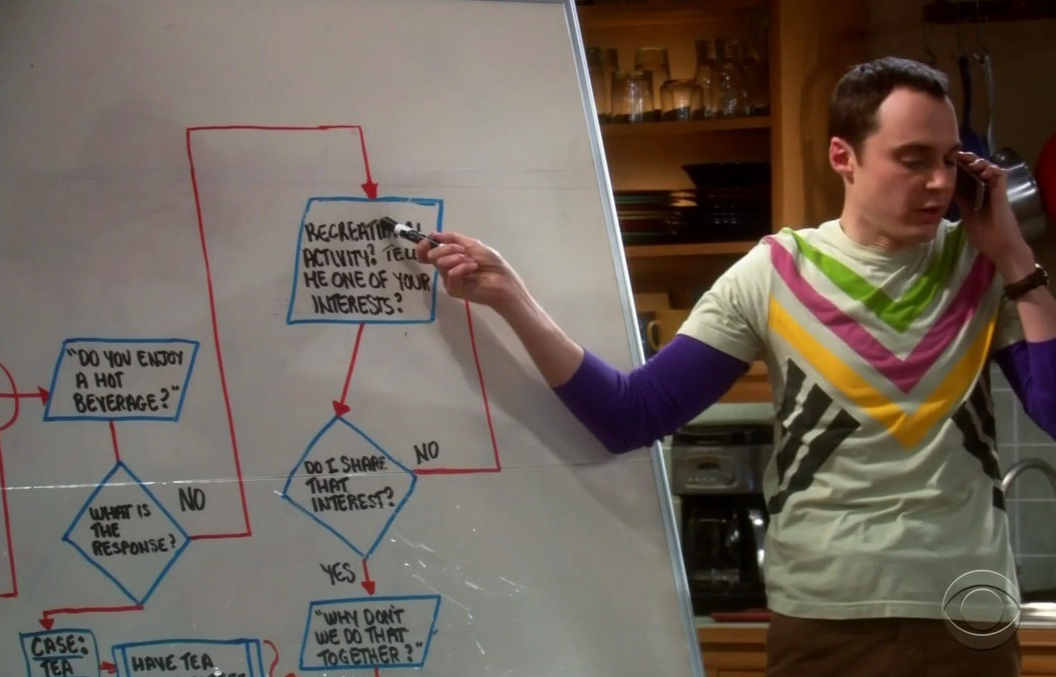
\includegraphics[width=7cm]{fig/Algorithm-sheldon.png}
            }
                 \textit{ I believe I've isolateblblblblblblsblbslbslbsl
            sblbslblsblsblblsblbs
            lbslblbslsb d the algorithm for making friends.}
     
            
            \small{
            \hfill Sheldon Cooper, 
            
            \hfill in \textit{The Big Band Theory}, Season 2, Episode 13
            }


    \end{columns}

\end{frame}


%%%%%%%%%%%%%%%%%%%%%
\subsection{Introduction}
    \begin{frame}
    \frametitle{Pourquoi faire appel � des algorithmes ?}
    Pour automatiser des t�ches
    
    Exemples :
    \begin{itemize}
    \item M�tier � tisser\\
    \item M�thode de calcul � la main d'une division\\
    \item Recette de cuisine\\
    \item ...\\
    \end{itemize}
    \end{frame}
 
 %%%%%%%%%%%%%%%%%
 
    \begin{frame}
    \frametitle{Qu'est-ce qu'un algorithme ?}
    \begin{block}{D�finition}
    Un algorithme est un ensemble 
    ordonn� d'instructions simples
permettant de r�soudre un probl�me.
    \end{block}
    \end{frame}
    
 %%%%%%%%%%%%%%%%%%
 \subsection{Construction d'un algorithme}
%%%%%%%%%%%%%%%%%%%    
\section{La machine de Turing}
%%%%%%%%%%%%%%%%%%%%
 
  
\begin{frame}[fragile]
\frametitle{Un peu d'histoire...}
\begin{codeblock}{Test}
\begin{codeC}
for (int i = 0 ; i < n ; i ++) {
    //a comment
    printf("%d",i);
    }
\end{codeC}
\end{codeblock}

\begin{termblock}{test 2}
\lstset{escapeinside={��}}
\begin{lstlisting}
�\textbf{>>}�./a.out
�\color{darkgray}{\texttt{  Hello World}}�
\end{lstlisting}
\end{termblock}

 \begin{block}{Bloc standard}
blablabla
\end{block}
\end{frame}


\begin{frame}[fragile]
\frametitle{essai}
\begin{columns}
\column{6cm}
\begin{block}

\begin{figure}
\begin{tikzpicture} [
    auto,
    decision/.style = { diamond, draw=blue, thick, fill=blue!20,
                        text width=5em, text badly centered,
                        inner sep=1pt, rounded corners },
    block/.style    = { rectangle, draw=blue, thick, 
                        fill=blue!20, text width=10em, text centered,
                        rounded corners, minimum height=2em },
    line/.style     = { draw, thick, ->, shorten >=2pt },
  ]
   \matrix [column sep=-10mm, row sep=10mm] {
                    & \node [text centered] (x) {$\mathbf{X}$};            & \\
                    & \node (null1) {};                                    & \\
                    & \node [block] (doa) {\textsf{DoAE}($\mathbf{X}$)};   & \\
  	               \node(null3){}; & \node [decision] (uiddes)
                        {\textsf{UID}($\hat{\mathbf{X}}$)};
                                  & \node[text centered](tra){$\mathbf{i}$}; \\
                  & \node [block] (track) {\textsf{DoAT}($\mathbf{x}$)}; & \\
                    & \node [block] (pesos)
                        {\textsf{BF}(DoA$_{\mathrm{T}}$,DoAs)};            & \\
                    & \node [block] (filtrado)
                        {\textsf{SF}($\mathbf{w}$,$\mathbf{x}$)};          & \\
                    & \node [text centered] (xf) {$\hat{x}(t)$ };          & \\
  };
  % connect all nodes defined above
 \begin{scope} [every path/.style=line]
    \path (x)        --    (doa);
    \path (doa)      --    node [near start] {DoAs} (uiddes);
    \path (tra)      --    (uiddes);
    \path (uiddes)   --++  (-3,0) node [near start] {no} |- (null1);
    \path (uiddes)   --    node [near start] {DoA} (track);
    \path (track)    --    node [near start] {DoA$_{\mathrm{T}}$} (pesos);
    \path (pesos)    --    node [near start] {\textbf{w}} (filtrado);
    \path (filtrado) --    (xf);
  
  \end{scope}
\end{tikzpicture}
\end{figure}
\end{block}
\column{3cm}
\begin{block}{bulbul}
\end{block}
\end{columns}
\end{frame}

\end{document}
